% =====================================================================
%  3.0 CONCEPTUAL DESIGN APPROACH  (55 pts)   P1.2, 31 Oct 2026
%  Rubric (5.1.4):  [x] Decomposition of mission reqs into subsystem reqs (3.1, Table 03)
%                   [x] Trade studies conducted, with results (3.3, Tables 04-05, Figs. 05-06)
%                   [x] Preliminary design / sizing results; concept sketch (3.4, Figs. 07-08, Table 06)
%                   [x] Sensitivity study of design parameters (3.2, Figs. 03-04)
%                   [x] Design approach per mission WITH initial targets (3.5, Table 07)
%  Numbers: data/p1.tex. Figures: tools/p1_figures.py. Table 03 clause sources: rules of 2 Sep 2026
%  (Secs. 3.1-3.3, 4.2). Table 04 evidence: DB-01 trades (analysis/out/trades_report.txt: audited matrices
%  with sensitivity weights; config_trades_report.txt) and DB-02 rev B (finalists, 30 Oct; S-06 airfoil;
%  A-04 tail and fail-safe). P1.2 applies the mock-judging notes of 31 Oct
%  (claude_docs/proposal_mock_judging_2026-10-31.md): one basis per table, alternatives shown,
%  Cm_alpha about the CG, the payload trades charted, the stow read as outside the window.
% =====================================================================
\needspace{4\baselineskip}
\section{Conceptual Design Approach}

% ---------------------------------------------------------------------
\subsection{Mission Requirements Decomposition}
Each mission score and rule became a numbered subsystem requirement (SR, Table~\ref{tab:decomp}); the SR column of Table~\ref{tab:tests} shows the test that verifies each.

\begin{table*}[t]
\caption{Mission requirements decomposed into subsystem requirements (SR). \textsuperscript{†}\,Team requirement beyond the rules.}\label{tab:decomp}
\begin{dbftable}{colspec={Q[l,wd=0.52in] Q[l,wd=1.08in] X[0.95,l] X[1.8,l]}}
Mission & Score & Key constraints & Derived subsystem requirements \\
M1 Staging & $M_1 = 1.0$ & 3 laps in 5 min; may be waived and credited by a successful M2 & SR-01 static margin \nStaticMargin\,\% MAC in every loading\textsuperscript{†}; SR-02 all checks inside the 5-min staging \\
M2 Delivery & $M_2 = 1 + \frac{W/t}{(W/t)_{\max}}$ & Container plus simulators at the declared maximum; TOP up; 5 laps & SR-03 bay for a 288\,$\times$\,303\,$\times$\,303~mm container; SR-04 positive restraint; SR-05 CG inside marked limits in every loading \\
M3 Sensor & $M_3 = 2 + \frac{N W_s}{(N W_s)_{\max}}$ & Internal until deployed, before the first downwind turn; OFF, SOLID, FLASHING, OFF; stow to land & SR-06 internal drum, tow $\geq$ \nTow~m, latched stow; SR-07 three lights, modes over the line, visible in sun; SR-08 no divergent swing at $n$ = \nMthreeN; SR-09 own COTS battery; SR-10 line clear of propeller, tail\textsuperscript{†}; SR-11 same door state every mission \\
Ground & $GM = 0.5 + \frac{W_s h}{(W_s h)_{\max}}$ & 6 drops on concrete, $h \leq$ 1.524~m (60~in); ring to bottom $<$ 381~mm (15~in); 5-min rigging & SR-12 container absorbs $W_s h$, sensor designed for 150~g; SR-13 tool-less O/E rigging, flush fittings; SR-14 test box drives all three modes \\
System & -- & Span $\leq$ 1.829~m (6~ft); TOGW $<$ 24.95~kg (55~lb); $\leq$ 100~Wh; no autopilot, GPS or camera; arming, fuse, radio rules & SR-15 pilot-in-the-loop only; SR-16 positive latches, no magnets; SR-17 §4.2.5 fail-safe, range check; SR-18 structure for $n$ = \nMthreeN{} and tip lift; SR-19 top arming plug $\geq$ 152~mm aft of the propeller plane, external Rx switch, separate Rx pack, BEC off, fuse $\leq$ pack rating; SR-20 M2 at full payload within \nUsableWh~Wh usable, stall $\leq$ 12~m/s; SR-21 ESC, pack within rated temperature\textsuperscript{†} \\
\end{dbftable}
\end{table*}

% ---------------------------------------------------------------------
\subsection{Scoring Model and Sensitivity Study}
The mission score sums four terms, each a completion credit plus a ratio to the best result in the field, our own included:\footnote{AIAA, \emph{2026--27 Design, Build, Fly Rules}, 2 Sep.~2026, Secs.~3.1--3.3, 6.3.}
\begin{equation}
\begin{aligned}
S_\mathrm{M} &= M_1 + \Bigl[1 + \tfrac{(W/t)}{(W/t)_\mathrm{max}}\Bigr]
  + \Bigl[2 + \tfrac{N W_s}{(N W_s)_\mathrm{max}}\Bigr] \\
 &\quad + \Bigl[0.5 + \tfrac{W_s h}{(W_s h)_\mathrm{max}}\Bigr] \leq 7.5
\end{aligned}
\end{equation}
Completion is worth 4.5 points and the bonuses at most 3.0, yet in 2026 only 17 of 83 inspected teams completed every mission;\footnote{AIAA, ``DBF Competition Summaries,'' 2022--2026 (513 team results).} winning totals ran \sWinLo--\sWinHi{} in 2022--26. The declared sensor mass $W_s$ sets the Ground Mission product, every Mission~2 container and the Mission~3 ballast cap.

Each design flies 120 random draws of every uncertain input (mass, $C_{L,\max}$, drag, efficiency, density and a lap-time factor from 24 measured flights\footnote{Predicted and measured times in seven DBF design reports, 2021--26; airframe masses of 14 top-three aircraft, 2022--26.}) against 5{,}000 simulated rival fields with attempt success from 2023--26; these inputs describe pilots and staging, not the payload, so they carry over and are refitted to the prototype's laps (TC-10). Efficiency, airframe mass and span efficiency lead the design parameters (Fig.~\ref{fig:sens}; \tEtaDn, \tMassUp{} and \tSpanEDn{} points per 10\,\%), and 10\,\% slower laps cost \tLapUp. Mission~2 uses \nMtwoWh{} of the \nUsableWh~Wh usable, leaving the 20\,\% reserve untouched. Declaring at inspection is the largest lever (Fig.~\ref{fig:declared}): fixed at design the best is \tFrozenBest{} (\tFrozenM~kg); declared, \sTotal{} with every mission completed.

\begin{figure}[t]
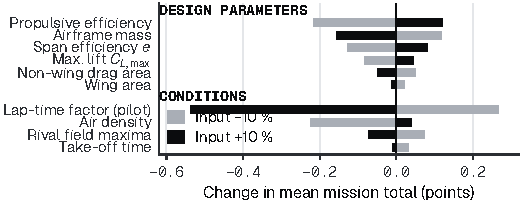
\includegraphics{figures/fig_tornado.pdf}
\caption{Mean mission total change for $\pm$10\,\% on each input: lap time and density, which the team does not set, outweigh every design parameter.}\label{fig:sens}
\end{figure}

\begin{figure}[t]
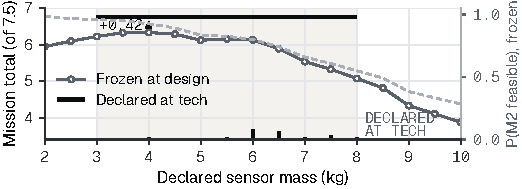
\includegraphics{figures/fig_declared.pdf}
\caption{Declaring at inspection is worth $+$\tDeclGain{} over the best mass fixed at design; fixed at 8~kg, Mission~2 is feasible on only \tFeasEight{} of airframes. Shaded: 3--8~kg window; bars: masses the draws declare.}\label{fig:declared}
\end{figure}

% ---------------------------------------------------------------------
\subsection{Configuration Trade Studies}
Trade weights come from the sensitivity study (completion \tCompletion\,\%, lap performance 17\,\%, high lift 10\,\%, airframe mass 7\,\%, efficiency 5\,\%, induced drag 4\,\%, structure and parasite drag 1\,\% each). The eleven best of 162 combinations of area, flap, declared range and propulsion were re-flown on all 120 draws (Fig.~\ref{fig:screen}) and had to hold Mission~3 completion within 10\,\% of the best and a worst-10\,\% total above the first iteration's. The 1.0~m² Fowler wing leads every finalist by \sTrailLo--\sTrailHi{} in P(top), the chance of the field's highest mission total, each paired 95\,\% interval above zero.\footnote{Flaps: R.~C. Platt, NACA Rept.~534, 1935; C.~J. Wenzinger and T.~A. Harris, NACA Rept.~664, 1939; method validated on NACA TN~663. Airfoils: M.~S. Selig et al., UIUC Low-Speed Airfoil Tests.} Table~\ref{tab:config} gives the other decisions: SD7037 is within 6\,\% of the best cruise $L/D$ of 13 sections (XFoil, $Re$ $5\times10^{5}$) and keeps its maximum lift tripped (UIUC), while the turn-lift leaders lose 15--52\,\% at $C_L$ 0.4. Fig.~\ref{fig:payload} and Table~\ref{tab:dr} give the payload and drum trades.

\begin{table}[t]
\caption{Configuration decisions. Points: change in mean mission total; matrix: weighted score of 100, team criteria weighted by the sensitivity study (top weights shown).}\label{tab:config}
\begin{dbftable}{colspec={Q[l,wd=0.50in] Q[l,wd=0.66in] X[l]}, colsep=3pt, cell{2-Z}{2}={font=\dbftotalrow}}
Decision & Selected & Alternatives, evidence \\
Planform & Straight & Delta $-$1.69, biplane $-$0.32 \\
Flap & Fowler, 1.0 & P(top) \sTrailLo--\sTrailHi{} lower \\
Airfoil & SD7037 & $L/D$ 73/92/96 at $C_L$ 0.4/0.6/1.0; trip-proof \\
 & & Of 13: E387 62/85/118, MH 114 35/64/119 \\
Wing & High, 90 & Low 71, mid 53 (bay 30\,\%, clearance 24\,\%) \\
Tail & Conv., 83 & T 73, twin boom 68 (line clearance 36\,\%); V: §4.2.5 fail-safe relies on mixing \\
Gear & Trike, 85 & Taildragger 76, bicycle 51 (landing 43\,\%) \\
Power & One 8S & 12S $-$0.02, twin $-$0.05 in P(top) \\
Tips & Plain & Winglets $-$0.01 to $-$0.05 \\
Sensor & At tech & Frozen $-$\tDeclGain{} (Fig.~\ref{fig:declared}) \\
\end{dbftable}
\end{table}


\begin{figure}[t]
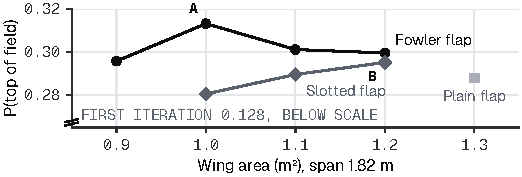
\includegraphics{figures/fig_screen.pdf}
\caption{Finalists on the same 120 draws: the 1.0~m² Fowler wing (A) leads; the slotted 1.2~m² wing (B) is the fallback. The axis starts at 0.265; each gap has its paired 95\,\% interval above zero.}\label{fig:screen}
\end{figure}

\begin{figure}[t]
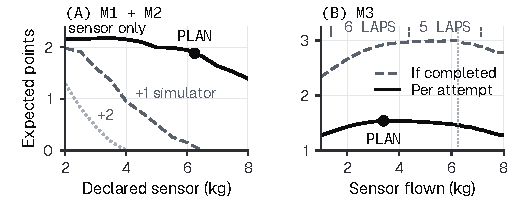
\includegraphics{figures/fig_payload.pdf}
\caption{Payload trades: (a) Mission 1 and 2 points against declared mass, 0 to 2 simulators; (b) Mission~3 points against sensor mass flown; dotted: 6.25~kg declared.}\label{fig:payload}
\end{figure}

\begin{table}[t]
\caption{Deployment-and-recovery trade (scores 1--5). Weights are the mission points at stake; the closed drum wins 99.5--100\,\% of 5{,}000 draws with estimates and weights randomised. Boom, wireless, bridle, pulley and spring reel failed the rules or the 20~s limit.}\label{tab:dr}
\begin{dbftable}{colspec={X[l] Q[c] Q[c,wd=0.42in] Q[c,wd=0.42in] Q[c,wd=0.42in]}, column{3}={bg=dbfAccentTint}, cell{1}{3}={bg=dbfInk, fg=white}, row{Z}={font=\dbftotalrow}, hline{Y}={0.4pt,dbfGraphite}}
Criterion & Wt. & Closed drum & Open drum & Free spool \\
Recovery reliability & 0.75 & 5.0 & 4.4 & 3.6 \\
Manufacturability & 0.15 & 3.1 & 5.0 & 1.7 \\
Weight, volume & 0.04 & 5.0 & 4.9 & 2.4 \\
Signal path & 0.03 & 5.0 & 5.0 & 5.0 \\
Deploy, stow time & 0.03 & 4.5 & 5.0 & 5.0 \\
Weighted total & 1.00 & \dbfselected{4.70} & 4.55 & 3.35 \\
\end{dbftable}
\end{table}

% ---------------------------------------------------------------------
\subsection{Preliminary Design and Sizing}
\subsubsection{Sizing method}
Sizing uses the hot-day density\fnRho{} of \nRho~kg/m³ and a lap model of the 152.4~m (500~ft) legs, 180° turns and downwind 360°, with stall $\leq$ 14~m/s, load factor $\leq$ 4, battery power, the 100~Wh cap and the measured $\times$1.15 lap factor. Mission~2 sits on its \nMtwoV~m/s, $n$ = \nMtwoN{} turn line at full thrust (Fig.~\ref{fig:constraint}); Mission~3 is energy-limited. Of 1{,}575 motor, propeller and pack combinations, 74 meet the turn limits and 40 were flown through the mission model; the AT7215 with a 20$\times$15E on 8S ranks first, 0.02--0.03 points ahead of a 21$\times$13E or a 12S pack, with \nThrust~N static thrust and \nPowerMtwo~kW (\nAmpsMtwo~A) mean power in Mission~2.\footnote{T-Motor and APC published test data; the model is within 3.5\,\% of a measured 2023 Mission~2 power.}

\begin{figure}[t]
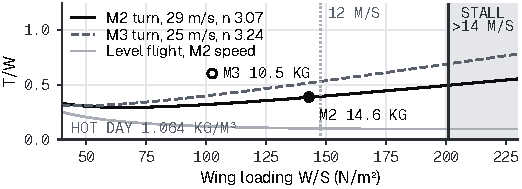
\includegraphics{figures/fig_constraint.pdf}
\caption{Mission~2 is sized by the race turn at full thrust; the Fowler flap keeps its \nGrossMtwo~kg landing under 12~m/s.}\label{fig:constraint}
\end{figure}

\begin{figure}[t]
\begin{dbfplate}{General arrangement / Variant A}{Span 1.82 m}
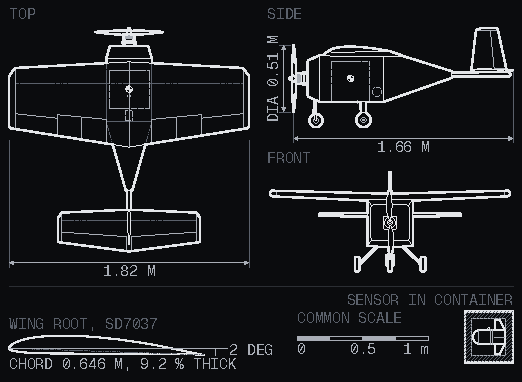
\includegraphics[width=\linewidth]{figures/fig_threeview.pdf}
\end{dbfplate}
\caption{Variant A to scale (AVL geometry; length from the propeller plane). Dashed: 8~kg container, drum, tow exit; quartered circle: CG. Below: wing root; sensor in its container.\gaStatus}\label{fig:concept}
\end{figure}

\subsubsection{Aircraft concept}
Variant A puts a straight wing (Fig.~\ref{fig:concept}, Table~\ref{tab:params}) on a 0.345\,$\times$\,0.355~m box fuselage with a conventional tail on a \nTailArm~m arm. The span sits 9~mm inside the 1.829~m limit (tip caps trimmed at weigh-in) and the area is the 1.00~m² of Fig.~\ref{fig:screen}, so the aspect ratio is \nAR. With the bay centred on the CG and the tow exit 50~mm aft, every loading flies at \nStaticMargin\,\% static margin; about the CG, AVL gives $C_{m\alpha}$ \nCma, $C_{n\beta}$ \nCnb{} and $C_{l\beta}$ \nClb{} per rad.\footnote{M.~Drela and H.~Youngren, AVL 3.52; M.~Drela, XFoil 6.99; MIT.} Variant B changes only the wing (1.2~m², slotted), tail and boom.

\begin{table}[t]
\caption{Design parameters, Variant A. Gross masses and stall speeds are medians of 120 draws, so they do not add up.}\label{tab:params}
\begin{dbftable}{colspec={X[l] Q[r] Q[l]}}
Parameter & Value & Unit \\
Span / area / aspect ratio & \nSpan{} / \nWingArea{} / \nAR & m, m² \\
Mean chord / tail arm & \nMAC{} / \nTailArm & m \\
Tail areas, H / V & \nSh{} / \nSv & m² \\
Empty mass with pack (fit) & \nEmptyMass & kg \\
Gross mass, M2 / M3 & \nGrossMtwo{} / \nGrossMthree & kg \\
Trimmed landing $C_{L,\max}$ & \nCLmaxLand & -- \\
Stall, M2 / M3 & \nStallMtwo{} / \nStallMthree & m/s \\
$C_{D0}$ / $L/D$, M2 level & \nCDzero{} / \nLDcruise & -- \\
Static margin / $C_{m\alpha}$ & \nStaticMargin{} / \nCma & \%, /rad \\
Static thrust / 8S pack & \nThrust{} / \nPackWh & N, Wh \\
M2 mean power / current & \nPowerMtwo{} / \nAmpsMtwo & kW, A \\
Tow line, built / minimum & \nTowDesign{} / \nTow & m \\
\end{dbftable}
\end{table}

\subsubsection{Sensor and D\&R system}
The sensor is a finned dart with a tungsten core (190~mm long, 85~mm body, 205~mm fins at 8~kg), towed from an eye above its CG so it flies level;\footnote{J.~Barrowman, ``Theoretical Prediction of the Center of Pressure,'' NARAM-8, 1966.} its potted electronics are designed for 150~g, checked by accelerometer in the drop tests, and a 1S pack drives three LED arrays of about 220~cd. A closed-loop servo drum (Table~\ref{tab:dr}) with a slip ring deploys 3.4~kg in about 10~s and stows it in \nStowMed~s (\nStowEight~s at 8~kg) into a latched dock. In a \nMthreeN~g turn the line carries \nTensionMed~N at 3.4~kg and \nTensionEight~N at 8~kg and is rated for four times the 3~g load. Towed 50~mm aft of the CG, the sensor keeps every loading at 16.0--16.1\,\% static margin; its 1.7~N trailing pull 0.18~m below the CG shifts $C_m$ by under 0.002 (estimate).

\subsubsection{Container and rigging}
Built once for the top of the range, the 288\,$\times$\,303\,$\times$\,303~mm container wraps the 205~mm fin span in 41~mm of polyethylene foam per face, keeping the sensor under 150~g in a 1.524~m drop with the ring under 381~mm from every face;\footnote{U.S. Dept.\ of Defense, \emph{MIL-HDBK-304B, Package Cushioning Design}, 1978.} pads are re-cut at inspection and simulators trim to 28~g.

% Targets table placed before 3.5 text so it lands before the 4.0 heading.
\begin{table}[t]
\caption{Mission targets: medians of 120 draws (P10--P90); design point in Section~3.5 (M2: \nMtwoTimeDP~s). Scores: means against the expected field, each mission completed.}\label{tab:targets}
\begin{dbftable}{colspec={Q[l,wd=0.46in] X[l] Q[r]}, row{X-Z}={font=\dbftotalrow}, hline{X}={0.4pt,dbfGraphite}, cell{X-Z}{1}={c=2}{l}}
Mission & Target & Score \\
M1 & Waived; credited by the first M2 & 1.00 \\
M2 & \nMtwoPayload~kg container; \nMtwoTime~s (\nMtwoTimeLo--\nMtwoTimeHi) & \sMtwo \\
M3 & \nMthreeMass~kg; \nMthreeProd~laps$\times$kg (\nMthreeProdLo--\nMthreeProdHi) & \sMthree \\
GM & \nDeclMed~kg from \nDrop~m: \nGMprod~kg$\cdot$m & \sGM \\
Total if completed, mean (P10) & & \sTotal{} (\sTotalPten) \\
Expected, failed attempts counted & & \sExpected \\
P(highest mission total) & & \sPtop \\
\end{dbftable}
\end{table}

% ---------------------------------------------------------------------
\subsection{Mission Design Approach and Scoring Targets}
Every plan protects completion first (Table~\ref{tab:targets}); speeds and times are the design point, not the medians.
\textbf{M1:} waived and credited by Mission~2, which lifts a typical team's chance of finishing Mission~3 from 0.40 to 0.72 (65\,\% per attempt, three attempts); Variant A's own chances are \sPMtwoDone{} (M2) and \sPMthreeDone{} (M3).
\textbf{M2:} one container and no simulators, since one at 6~kg is feasible in only \pSimFeas{} of draws and costs more completion than its $W/t$ earns (Fig.~\ref{fig:payload}a); \nMtwoV~m/s with \nMtwoBank° turns gives \nMtwoLap~s laps, \nMtwoTimeDP~s with take-off (median \nMtwoTime~s).
\textbf{M3:} lights OFF upwind, SOLID after lap~1, FLASHING after lap~2, OFF and stow after the last lap. Ballast is chosen per attempt (Fig.~\ref{fig:payload}b): the optimum is flat at \pMthreeLo--\pMthreeHi~kg because lighter darts stall slower and climb harder, so \nMthreeMass~kg flies \nMthreeLaps{} laps of \nMthreeLap~s at \nMthreeV~m/s. Charging the stow to the window costs only \pStowFree{} points.
\textbf{GM:} \nDeclMed~kg from \nDrop~m gives \nGMprod~kg$\cdot$m, above the expected field best (\sFieldGMexp) in most draws; rigging drilled under 240~s.
\textbf{Switch rule:} if the Fowler section gives trimmed $C_{L,\max}$ below 1.75, or jams more than once in 100 cycles, by 15~January, Variant B is built; it trails A by \sRegB{} in P(top) when the flap works and leads by \sRegA{} when it does not.
